\documentclass[10pt]{article} % For LaTeX2e
\usepackage{tmlr}
% Camera-ready: \usepackage[accepted]{tmlr}   Preprint: \usepackage[preprint]{tmlr}
\usepackage{amsmath,amssymb}
\usepackage{booktabs}
\usepackage{tabularx}
\usepackage{enumitem}
\usepackage{graphicx}
\usepackage{flafter}
\usepackage{tikz}
\usetikzlibrary{positioning,arrows}
\usepackage{hyperref}
\usepackage{url}
\hypersetup{hidelinks}
\raggedbottom

\newcommand{\rsix}{r6.2}
\newcommand{\rfour}{r4.2}

\def\month{09}
\def\year{2026}
\def\openreview{\url{https://openreview.net/forum?id=XXXX}}

\title{What Do Benign-Trained Session Language Models Actually Detect? \\ A Mechanistic Audit on Insider-Threat Benchmarks}

\author{\name Anonymous Authors \email anonymous@example.com \\
\addr Anonymous Institution}

\begin{document}

\maketitle


\begin{abstract}
High ranking performance does not reveal what an anomaly detector uses
to distinguish malicious activity from normal activity. We audit a language
model adapted only to benign employee logs by decomposing its internal
changes into sparse features, intervening on selected features, and
measuring where they activate. On CERT r6.2, the selected features activate
almost entirely at personality and organizational fields; on r4.2, four of
five concentrate on behavioral session fields. Comparing malicious days
only with benign users unseen during adaptation reduces day-level ranking
quality from $0.95$ to $0.55$ and from $0.96$ to $0.67$, respectively.
The attribution pattern survives new dictionaries and smaller-model
replications, while some intervention effects do not. A real-user study
with personality questionnaires supplies a behavioral counterpart; a real
authentication log shows a related generalization gap that is sensitive
to computer identifiers. Removing profile content from both adaptation
and scoring improves user-level ranking from $0.53$ to $0.90$ in the
audited Qwen3-8B run, with a smaller change in Qwen2.5-3B. These comparisons
use one adapter seed per condition and only four malicious CERT r6.2
users, so they establish a result for those runs rather than a general
capacity effect. The contribution is an audit that separates ranking
quality, causal relevance, and the input locations of selected features,
while making the limits of each measurement explicit.
\end{abstract}

\section{Introduction}
\label{sec:intro}

Organizations record what employees do on their computers: logons, file
transfers, web activity, e-mail volume, and so on. An \emph{insider
threat} is an employee who misuses legitimate access, for example by
stealing data. Because such events are rare, a common approach is
\emph{anomaly detection}: build a statistical model of normal activity,
and flag days that the model finds unusual.

Formally, a detector is a function $s$ that assigns a real-valued
\emph{anomaly score} $s(x)$ to each observation $x$, where in our
setting $x$ is a record of one user's activity on one day. Higher
scores are meant to indicate more suspicious activity. Detectors are
usually evaluated by how well their scores \emph{rank} malicious days
above benign ones. The standard summary of ranking quality is the
following probability, estimated over a labeled test set:
\begin{equation}
\mathrm{AUC} = \Pr\bigl(s(X_{\mathrm{mal}})>s(X_{\mathrm{ben}})\bigr)
+ \tfrac12\Pr\bigl(s(X_{\mathrm{mal}})=s(X_{\mathrm{ben}})\bigr),
\label{eq:auc}
\end{equation}
where $X_{\mathrm{mal}}$ is a randomly chosen malicious day and
$X_{\mathrm{ben}}$ a randomly chosen benign day. (This quantity is
commonly called the ROC-AUC, for ``area under the receiver operating
characteristic curve''; the probability formulation is equivalent and is
the only form we need; ties receive half credit.) An AUC of $1$ means perfect ranking and $0.5$
means this ranking measure equals its chance reference.

The question that motivates our work is simple to state. A high AUC
says that the score \emph{separates} the two classes. It does not say
\emph{on the basis of what information} the separation is achieved. Two
detectors with identical AUC could work very differently: one might
respond to genuinely unusual behavior, while the other might respond to
incidental properties of \emph{who} the malicious users happen to be,
such as their role, department, or personality profile. Such a shortcut can fail when the relationship between identity and
malicious activity changes, including when the detector encounters new users. This paper develops a
method for determining which kind of detector one actually has, applies
it to a modern detector built from a large language model, and then
subjects the answer to a systematic robustness program.

This question connects anomaly detection \citep{chandola2009anomaly}
with shortcut learning \citep{geirhos2020shortcut,lapuschkin2019unmasking}:
good predictions can rely on unintended cues. Security evaluation also
requires careful control of data splits and experimental assumptions
\citep{arp2022dos,landauer2024critical}. Our contribution is the combined
audit of adaptation changes, feature interventions, input locations, and
user-disjoint evaluation; we do not introduce a new sparse-coding method
or claim a detection leaderboard advance. Section~\ref{sec:related}
places this combination alongside earlier log detectors and interpretability
methods.

\paragraph{Contributions.}
\begin{enumerate}[leftmargin=1.3em]
\item An audit for benign-adapted anomaly language models that separates
three questions a score cannot: whether a detector ranks well, which selected
internal directions affect its score (a sparse dictionary over
adapter-induced changes, repair and ablation against active controls,
user-level uncertainty, same-user exclusion), and where those directions
activate in the input (Sections~\ref{sec:detector}--\ref{sec:method}).
\item On two CERT benchmarks with nearly identical ranking quality, the
audited detectors rest on different selected evidence: profile positions on
r6.2 ($99.8$--$100$ percent of the selected features' activation mass) and
session positions on r4.2. Comparing malicious days only with benign users
unseen during adaptation reduces day-level AUC from $0.95$ to $0.55$ and from
$0.96$ to $0.67$ (Section~\ref{sec:findings}). The attribution pattern
survives new dictionaries, benign-only dictionaries, and smaller-model reruns;
some intervention effects do not (Section~\ref{sec:robustness}).
\item Two real-data tests and a cross-detector comparison: real users with
real personality questionnaires (TWOS) give a behavioral counterpart with
within-user AUC $0.78$; a raw enterprise authentication log with no profile
(LANL) shows a seen-versus-unseen gap that cannot yet be attributed,
because its evaluation pools differ in user composition as well as training
exposure; classical one-class detectors given the same
r6.2 profile columns show little profile reliance
(Sections~\ref{sec:realdata}--\ref{sec:classical}).
\item A train-matched serialization experiment: removing profile content from
adaptation and scoring raises unseen-user ranking from $0.53$ to $0.90$ in
the audited Qwen3-8B run (descriptive paired interval excluding zero), with a
small, non-significant change in the audited Qwen2.5-3B run; shuffling
profiles into stable pseudonyms never helps while profile-dominated features
persist, so capture and harm are different things
(Section~\ref{sec:factorial}).
\end{enumerate}

\section{Related work}
\label{sec:related}

\emph{Insider-threat detection.} The CERT datasets
\citep{glasser2013bridging,certdataset} are the standard public benchmarks;
prior detectors range from unsupervised deep models over aggregated user-day
features \citep{tuor2017deep,le2020analyzing,yuan2021deep} to one-class
methods such as Deep SVDD \citep{ruff2018deepsvdd} and Isolation Forest
\citep{liu2008isolation}, which serve as our baselines.
\emph{Language models over logs.} Sequence models for log anomaly detection
predate current large language models \citep{du2017deeplog,guo2021logbert};
benign-trained event-level language models over authentication logs
condition on user identity by construction \citep{tuor2018recurrent}, and
LoRA-tuned and LLM-based insider-threat systems are now being built
\citep{song2025dmfi,sun2025redchronos}. Facade \citep{kantchelian2024facade}
names the pathology in which a detector separates classes by featurizing
actions through the token of their principal and engineers around it on
proprietary data; we instead open a benign-trained detector on public data
and characterize the shortcut.
\emph{Mechanistic interpretability.} Sparse autoencoders decompose
activations into sparse features
\citep{cunningham2023sparse,bricken2023monosemanticity,gao2024scaling};
activation patching and ablation supply causal tests
\citep{vig2020investigating,meng2022locating,zhang2023best,heimersheim2024use},
with causal scrubbing as the formal standard \citep{chan2022causal}. Feature
identity can split or be absorbed across dictionaries
\citep{chanin2024absorption}, and LoRA delta activations have been analyzed
with sparse autoencoders \citep{prasanth2026lora}. We follow the
recommendation to measure effects against matched controls
\citep{zhang2023best} and treat cross-dataset transfer as an empirical claim
\citep{olah2020zoom,chughtai2023toy}.
\emph{Shortcuts and evaluation pitfalls.} Our finding is an instance of
shortcut learning
\citep{geirhos2020shortcut,lapuschkin2019unmasking,damour2020underspecification},
previously shown for anomaly detectors through input attribution
\citep{kauffmann2020clever}. User-disjoint evaluation and profile masking are
the evaluation hygiene that security work prescribes \citep{arp2022dos}, and
the seen-versus-unseen collapse is the identity-leakage analogue of benchmark
critiques for log anomaly detection \citep{landauer2024critical}.

\section{Data and serialization}
\label{sec:data}

We use two versions, r4.2 and r6.2, of the CERT insider-threat
corpus, a synthetic enterprise dataset produced by Carnegie Mellon
University \citep{certdataset,glasser2013bridging}. Raw activity is aggregated
into session features following the approach of \citet{le2020analyzing},
then grouped into user-days. Our evaluation covers only days represented
in those extracted sessions. This distinction changes the population:
r6.2 has $70$ positive user-days from $4$ malicious users in our matched
domain, compared with $99$ positive answer-key rows from $5$ users;
r4.2 has $1{,}309$ days from $60$ users, compared with $1{,}883$ rows from
$70$ users. Incidents outside session coverage are not evaluated.
We later examine two real datasets, TWOS and LANL
(Sections~\ref{sec:twos} and~\ref{sec:lanl}).

Each user-day is converted into a short structured text with three
kinds of lines:
\begin{itemize}
\item a \texttt{DAY} line holding the week and organizational fields for that
user (project, role, business unit, department, team, and an
information-technology administrator flag);
\item a \texttt{PSY} line holding the user's five simulated personality
scores. These are the ``Big Five'' personality traits used in
psychology: openness (O), conscientiousness (C), extraversion (E),
agreeableness (A), and neuroticism (N). In CERT these numbers are
generated by the simulator and are constant for each user;
\item one \texttt{SES} line per work session, holding numeric
behavioral counts for that session: duration, number of logons, file
and removable-drive activity, e-mail volume, web-browsing category
counts, and similar quantities.
\end{itemize}
A user-day text is therefore a small table serialized as text. The
first two lines contain the profile fields, most of which are constant
across a user's days, while the session lines describe daily activity.
The text also contains a session-count line, labeled \texttt{SESCOUNT}. We use \emph{profile} for the \texttt{DAY}/\texttt{PSY} classes
and \emph{behavioral} for \texttt{SES}; these are locations in the input,
not assumptions about the exact computation represented there. This
partition of the input is the reference frame for the entire paper.

Users are split as follows. Users with any malicious day are reserved
entirely for evaluation. The remaining benign users are divided into a
training set (roughly ninety percent) and a validation set (roughly ten
percent) whose days never enter training. The validation users will
play an important role: they provide a comparison group absent from adaptation. Some scored
evaluation users also have no positive day within the matched domain;
Appendix~\ref{app:populations} specifies the populations used in each test.

\section{The detector}
\label{sec:detector}

\subsection{Language models as probability distributions}

A \emph{language model} is a parametric probability distribution over
sequences of symbols called tokens. Writing a sequence as
$x = (x_1, \dots, x_n)$, the model has the product form
\begin{equation}
p_\theta(x) \;=\; \prod_{t=1}^{n} p_\theta\bigl(x_t \mid x_1, \dots,
x_{t-1}\bigr),
\end{equation}
where each conditional distribution is computed by a neural network
with parameters $\theta$. Modern large language models are such
networks with billions of parameters, trained on enormous general text
corpora. We use Qwen3-8B, an eight-billion-parameter model \citep{qwen3}. The
network processes a sequence through $L$ successive layers; at layer
$\ell$ and position $t$ it maintains an internal state vector
$h^{(\ell)}_t \in \mathbb{R}^{d}$ with $d = 4096$. These internal
vectors matter later: they are the objects we analyze.

\subsection{Adapting the model to normal behavior only}

We specialize the general-purpose model to our corpus by
\emph{fine-tuning}: continuing its training on the serialized user-day
texts, using only days from benign training users. The objective is
maximum likelihood, that is, minimizing the negative log-likelihood of
the benign corpus $\mathcal{D}$:
\begin{equation}
\mathcal{L}(\theta) \;=\; -\sum_{x \in \mathcal{D}} \sum_{t}
\log p_\theta\bigl(x_t \mid x_{<t}\bigr).
\end{equation}
No malicious example is ever used in training. This is the classical
one-class setup: model the normal population, then measure deviation
from it.

For efficiency the fine-tuning does not modify all eight billion
parameters. Each adapted attention or feed-forward projection matrix $W$ is kept fixed and
receives a trainable low-rank correction,
\begin{equation}
W' \;=\; W + \tfrac{\alpha}{r} BA, \qquad
B \in \mathbb{R}^{d_{\mathrm{out}} \times r},\;
A \in \mathbb{R}^{r \times d_{\mathrm{in}}},
\end{equation}
with rank $r = 16$, so only the small matrices $A$ and $B$ are learned.
This technique is called LoRA (low-rank adaptation) \citep{hu2022lora}; we use a
memory-saving variant called QLoRA in which the fixed weights are
stored at reduced numerical precision \citep{dettmers2023qlora}. The pair (fixed base model,
learned low-rank correction) is called the \emph{adapted model}. The
important point is that the learned weight updates are carried by
removable low-rank adapters, which makes before-versus-after
comparisons clean.

\subsection{The anomaly score and two ways to evaluate it}
\label{sec:protocols}

The score of a day $x$ is its average surprisal under the adapted
model:
\begin{equation}
s(x) \;=\; -\frac{1}{n-1}\sum_{t=2}^{n} \log
p_{\theta_{\mathrm{ada}}}\bigl(x_t \mid x_{<t}\bigr).
\end{equation}
Here the first input token supplies context; the remaining tokens are
scored as next-token targets, with padding excluded. Days that the model
of normal behavior finds improbable receive high scores.

We compare two evaluation populations. Their difference is part of
the finding, because they ask different questions about generalization.
\begin{enumerate}
\item \emph{The original fold-aligned comparison.} Malicious days are compared against
benign days drawn from the general population. Because the model was
trained on about ninety percent of benign users, most of those benign
comparison days belong to users the model saw during training. Under
this protocol the adapted model looks excellent: AUC about $0.953$ on
r6.2 and $0.964$ on r4.2, higher than four standard anomaly-detection
baselines evaluated on the same benchmarks (an isolation forest, a
deep one-class method called Deep SVDD, and two
recurrent autoencoders), whose AUC values range from about $0.63$ to
$0.77$. Here a fold contains one malicious user and $800$ benign users.
The language model is held fixed across folds, whereas the baselines
retrain with those test users excluded: the training exposure is unequal.
\item \emph{The user-disjoint protocol.} Malicious days are compared
only against benign days of the validation users, whom the model never
saw. Malicious users are unseen by construction, so under this protocol
neither side contributes user-days to adaptation.
\end{enumerate}
The second comparison removes the imbalance in training exposure.
It does not make unseen profiles identical across classes or isolate
familiarity from every other population difference. We report the gap in
Section~\ref{sec:collapse} and test profile sensitivity separately.

AUC also does not specify how many alerts are correct. We therefore report
\emph{average precision} (AP), which averages precision as the score
threshold admits more positives. The result plots label this quantity
PR-AUC, following the evaluation code. Its random-ranking reference is
the positive fraction of the evaluated population; it is not precision
at a single operational threshold. Appendix~\ref{app:detectors} gives the
full baseline comparison.

\section{Opening the model}
\label{sec:method}

We now describe the four analysis steps, in the order they are applied.
Together they connect the model's internal changes to measurable
score effects and input locations.

Figure~\ref{fig:architecture} summarizes the sequence.

\input{figures/architecture_linear.tex}

\subsection{Step 1: isolate what fine-tuning changed}

Because the base model is kept frozen, we can run the same day $x$
through both the base and adapted models and subtract their internal
states. Define, at a chosen layer $\ell$ and each token position $t$,
\begin{equation}
\delta_t \;=\; h^{(\ell), \mathrm{ada}}_t - h^{(\ell),
\mathrm{base}}_t \;\in\; \mathbb{R}^{d}.
\end{equation}
The vector $\delta_t$ isolates the representational change induced by
the adaptation at the audited layer and position. It is the natural
object to study if one wants to know what the adaptation, as opposed to
the general-purpose model, contributes at that point in the
computation.

\subsection{Step 2: approximate the changes with a sparse dictionary}

The vectors $\delta_t$ live in $\mathbb{R}^{4096}$ and are not
individually interpretable. We therefore approximate them by sparse
nonnegative combinations of learned dictionary elements. After
standardizing each coordinate (subtracting its mean $\mu$ and dividing
by its standard deviation $\sigma$), we seek a dictionary matrix
$D \in \mathbb{R}^{d \times m}$ (with $m$ columns, called \emph{features};
$m = 4d$ for the headline r6.2 audit and $m = 2d$ for the native r4.2 audit) and, for each standardized vector
$\tilde\delta_t$, a coefficient vector
$z_t \in \mathbb{R}^{m}_{\geq 0}$ with at most $k$ nonzero entries ($k = 8$
and $k = 4$ respectively), such that
\begin{equation}
\tilde\delta_t \;\approx\; D z_t ,
\end{equation}
with $D$ and the coefficients chosen to minimize the mean squared
reconstruction error over a large sample of token positions. This is a
sparse coding problem; the particular parametrization we use (a
one-layer encoder network followed by a keep-the-largest-$k$ rule and a
linear decoder) is called a \emph{sparse autoencoder} in the
machine-learning literature \citep{cunningham2023sparse,gao2024scaling}. The outcome is that each change vector is
expressed as a short combination of reusable directions, and each
direction can be studied on its own. One technical point deserves
notice: because the standardization constants differ between datasets,
any geometric comparison of features across datasets must first map the
dictionary columns back to the original coordinates, that is, compare
the directions $\sigma \odot D_{:,f}$ rather than the raw columns. All
cross-dataset comparisons in this paper do so.

\subsection{Step 3: select the score-relevant features and test them
causally}
\label{sec:interventions}

We use a simple screening rule to propose candidate features: the
difference in mean activation between malicious and benign token rows.
A small mean difference does not rule out a more complex contribution.
The ranking statistic is
\begin{equation}
g_f \;=\; \mathbb{E}\bigl[z_{t,f} \mid \text{malicious day}\bigr] -
\mathbb{E}\bigl[z_{t,f} \mid \text{benign day}\bigr],
\end{equation}
and we take the five features with the largest $g_f$ as the candidate set
$S$. As a comparison group we also select a matched \emph{control} set
$C$ of five features with nontrivial activation frequency and a small
absolute gap $|g_f|$. This active control avoids comparison with features
that never fire; closer matching of edit magnitude is a separate check. Selection by a statistic can be
flattered by chance, so everything that follows treats $S$ as a
hypothesis to be tested rather than a conclusion.

The test is interventional. The idea is to edit the coefficients of the
selected features inside the model, let the edited internal state flow
through the remaining layers, and observe whether the anomaly score
responds. We use two complementary edits.

\emph{Repair (a sufficiency-style test).} For a malicious day, we move
the selected coefficients toward the values they take on a comparable
benign day (a ``donor'' from the same organizational context, never the
same user), with an interpolation strength
$\alpha \in \{0.25, 0.5, 0.75, 1\}$, and record the best achievable
repair over the available donors and strengths. Write
$\Delta^{S}_{\mathrm{ben}}$ for the best \emph{signed score change},
$s_{\mathrm{edited}}-s_{\mathrm{original}}$, so a reduction is negative, and
$\Delta^{S}_{\mathrm{anom}}$ for the analogous quantity when donors are
other malicious days. If the selected features carry anomaly-specific
repairable structure, moving them toward benign values should reduce
the score more than moving them toward other anomalous values, and it
should do so more for $S$ than for the control set $C$. The reported
estimand is the doubly differenced quantity
\begin{equation}
\tau \;=\; \bigl(\overline{\Delta^{S}_{\mathrm{anom}}} -
\overline{\Delta^{S}_{\mathrm{ben}}}\bigr) -
\bigl(\overline{\Delta^{C}_{\mathrm{anom}}} -
\overline{\Delta^{C}_{\mathrm{ben}}}\bigr).
\end{equation}
Each bar averages the same receivers with all four required outcomes.
This paired construction avoids subtracting means over different subsets
when donors are missing. It controls some generic effects of editing,
but unequal edit sizes and nonlinear responses need not cancel. Because each
receiver keeps its best candidate, $\tau$ describes the best of the searched
edits, not a typical edit: on r4.2's held-out users the same contrast averaged
over donors has the opposite sign (Section~\ref{sec:robustness}). Each edit is
also joint: every selected coefficient is written at the union of the set's
active positions, including coefficients that were zero there.
The operation also replaces the original delta with its sparse
reconstruction at every token in both arms. That shared replacement
is not a guarantee of exact cancellation; the equations and sensitivity
checks are in Appendix~\ref{app:intervention}.

\emph{Ablation (a necessity-style test).} We scale the selected
coefficients toward zero, on malicious days and on matched benign days,
and ask whether removal disrupts the score more on the malicious side
and more for $S$ than for $C$. The corresponding double difference is
denoted $\nu$; its signed definition is in Appendix~\ref{app:intervention}.
A positive repair contrast shows that some searched edit of the set is
useful given the rest of the network, and ablation establishes dependence
under that edit. Neither
proves that a feature set is sufficient by itself or strictly necessary
in a network with redundant pathways \citep{heimersheim2024use,zhang2023best}.

Two safeguards are essential and were arrived at the hard way. First,
donors from the same user are excluded: allowing them lets the
procedure ``repair'' a malicious day by borrowing the same person's own
benign signature, which inflates effects for reasons unrelated to the
question. Second, uncertainty is computed by resampling \emph{users},
not days: multiple days of the same user are statistically dependent,
so the primary intervention intervals resample malicious users with
replacement ($10{,}000$ draws) and recompute the paired effect.
The masking analysis resamples users within both label groups.
Intervals are conditional on the trained models and selected configurations. On r6.2, which has only four malicious users, such intervals
are reported as descriptive.

One further check matters because the selected features are, by
construction, strongly activated: their edits are physically larger
than edits of the control features. We therefore repeated the headline
comparisons with \emph{proxy-matched} controls, chosen to match the
selected features on activation frequency, activation magnitude, and
standardized dictionary-direction norm, which narrows the edit-size gap to a
factor of $1.3$ to $1.8$. The proxies do not use the realized coefficient
changes, the standardization factor of the actual patch, or the edited
positions, so this is not an equal-perturbation test. The contrasts survive: on r4.2 the repair contrast
remains clearly positive ($+0.0017$ with interval $[0.0011, 0.0023]$)
and on r6.2 the ablation contrast remains clearly positive ($+0.061$
with interval $[0.007, 0.084]$); the remaining two contrasts stay
positive but with intervals containing zero. Matching reduces rather
than eliminates the difference in edit strength. Dividing effects by
edit norm gives a less favorable r6.2 repair result; that sensitivity
is retained in Appendix~\ref{app:intervention}. Figure~\ref{fig:effects}
summarizes the intervention measurements.

\begin{figure}[t]
\centering

\includegraphics[width=\textwidth]{figures/mech_effects.pdf}
\caption{Effect of editing the selected features, compared with editing
matched control features, on the anomaly score (one panel per benchmark
and per type of edit; units are thousandths of the score). Each point
is the average paired contrast for one organizational matching context, and each
horizontal bar is a $95$ percent confidence interval computed with the
malicious users as the resampling unit. Positive values favor the selected set in the specified
donor-type or receiver-class contrast, relative to the active control. Open circles mark intervals that include zero.}
\label{fig:effects}
\end{figure}

\subsection{Step 4: read off what the features respond to}

Finally we ask \emph{where} the selected features activate within the
day text. Each token position belongs to \texttt{DAY}, \texttt{PSY},
\texttt{SESCOUNT}, or \texttt{SES}. The fractions below are computed
over positive-example token rows. For a feature $f$, define its
\emph{attribution mass} on class $c$ as the fraction of its total
activation that occurs at positions of that class:
\begin{equation}
m_f(c) \;=\;
\frac{\sum_{(x,t)\,:\, \mathrm{class}(t) = c} z_{t,f}(x)}
     {\sum_{(x,t)} z_{t,f}(x)} .
\end{equation}
Profile-position mass is $m_f(\texttt{DAY})+m_f(\texttt{PSY})$;
behavioral-position mass is $m_f(\texttt{SES})$. We also compare each
fraction with the fraction of tokens at that location, so that a long
line class does not receive credit merely for occupying more of the input.

These measurements answer different questions. Interventions test whether
editing a selected set changes the score. Attribution locates where that
set activates. A hidden state at a session token can still depend on
an earlier profile, so location does not fully identify a feature's
meaning. Nor are the five selected features a complete account of the
model: $100$ percent profile mass within them is not $100$ percent of
the detector's decision. We use input-level swaps, masking, and
within-user evaluation to help interpret the combined evidence.

\section{Findings on the two CERT benchmarks}
\label{sec:findings}

\subsection{Similar ranking, different selected features}

The two CERT versions produce nearly identical headline AUC values, yet
the analysis finds qualitatively different selected feature sets.

On r6.2, the five selected features place between $99.8$ and $100$
percent of their attribution mass on the personality and organizational
lines, with activation on the personality line enriched about thirteen
times over its share of tokens. The intervention contrasts are positive
(repair $\tau = 0.0068$ with descriptive interval $[0.0001, 0.0100]$;
ablation $\nu = 0.065$ with interval $[0.026, 0.083]$). The five gap-ranked features concentrate on profile positions; their
intervention contrast is evidence of score relevance, not a ranking of
the five largest individual causal effects.

On r4.2, four of the five selected features concentrate on the
behavioral session lines (the fifth responds to the organizational
header). The contrasts are again positive (repair $\tau = 0.0014$ with
interval $[0.0010, 0.0019]$; ablation $\nu = 0.0029$ with interval
$[0.0009, 0.0050]$). The selected set therefore concentrates on the session portion of the input.
Splitting the loss change of the held-out r4.2 edits by the class of the
predicted token (Appendix~\ref{app:pkg4}) shows that, at the larger
strengths, the selected edits raise behavior-token loss more than control
edits do ($+0.016$ to $+0.018$ nats per token with benign donors at full
strength, every interval excluding zero). Their differential effect on
profile-token loss is uncertain, and the preregistered direct comparison of
the two classes is inconclusive. This is evidence about a joint edit under
the SAE replacement procedure. It does not show that the features represent
malicious behavior, that the effect exceeds an equally large perturbation at
the same positions, or that it is specific to anomalous days, since every
receiver was a malicious day. Figure~\ref{fig:attribution} shows the contrast, together with
the real-data result of Section~\ref{sec:twos}.

\begin{figure}[t]
\centering
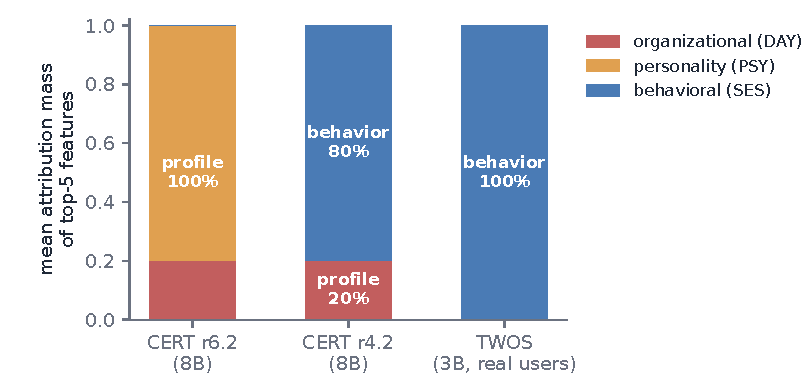
\includegraphics[width=0.85\textwidth]{figures/attribution_summary.pdf}
\caption{Where the selected features place their activation, averaged
over each detector's five selected features. Each bar decomposes the
activation mass into the organizational lines, the personality lines,
and the behavioral session lines of the input text. The selected features concentrate on profile positions in r6.2 and
on session positions in r4.2 and TWOS. These are averages over features,
not shares of the whole model's decision.}
\label{fig:attribution}
\end{figure}

\subsection{The consequence for the headline numbers}
\label{sec:collapse}

Why would reading a user's static profile produce a high AUC at all?
The adapted model was trained on roughly ninety percent of the benign
users. For those users, the model has been repeatedly exposed to the
constant profile lines, which may make those profiles easier to predict. The malicious users
were never seen in training, so unfamiliar profile text could raise
their scores even without unusual activity. This offers a familiarity
hypothesis for some of the score gap,
which the following comparisons test.

The user-disjoint protocol of Section~\ref{sec:protocols} removes this
asymmetry, and the effect is large. The AUC falls from $0.954$ to
$0.545$ on r6.2, which is barely better than chance, and from $0.959$
to $0.668$ on r4.2. These values fall below the baselines' original fold-aligned AUCs;
because the populations differ, this is evidence against a detector
superiority claim rather than a new controlled leaderboard. Two further
measurements complete the picture. First, ranking each malicious user's
own days (their malicious days against their own benign days, identity
held fixed) still succeeds moderately on both benchmarks (average
within-user AUC $0.67$ on r4.2 and $0.73$ on r6.2), so the score contains variation within identities that a static
profile-only score could not supply. The within-user intervals and
counts are given in Appendix~\ref{app:detectors}. Second, deleting the personality lines from the
inputs at scoring time \emph{improves} the r4.2 detector's performance
on unseen users from $0.67$ to about $0.80$ (an increase of $0.127$
with interval $[0.061, 0.193]$): including the profile text lowered discrimination in that
fixed-adapter comparison. On r6.2,
the masking contrasts have intervals spanning zero. This experiment
does not show that all profile information is uninformative or that
behavioral information is absent; the within-user result already rules
out the latter extreme. The masking population and all three conditions
are specified in Appendix~\ref{app:detectors}.
Figure~\ref{fig:collapse} shows the baseline comparison and the
collapse.

\begin{figure}[t]
\centering

\includegraphics[width=\textwidth]{figures/detector_dissociation.pdf}
\caption{Score-level results. Left and center panels: ranking quality
(vertical axis) and average precision (horizontal axis, logarithmic scale) for
the language-model detector (blue) and four standard anomaly-detection
methods on the two benchmarks; the language model attains the highest
ranking quality under the original fold-aligned protocol.
The baseline abbreviations are expanded in Appendix~\ref{app:detectors}. Right panel: the same
language-model ranking quality when malicious users are compared only
against benign users never seen during training. The apparent advantage
largely disappears, and the dashed line marks chance level.}
\label{fig:collapse}
\end{figure}

\subsection{Can the same features be reused across benchmarks?}

Directly applying the r6.2 dictionary and feature sets to r4.2 fails:
the repair contrasts are negative across all audited transfer
configurations, with best values around $-0.001$. Searching within r4.2
instead finds the positive layer-26 result above. The audit can therefore
be reused, but the same sparse features did not transfer in these runs.
Seed and matched-layer comparisons below test whether this failure is
simply an accident of dictionary initialization. A local session
autoencoder supplies another comparator, but its score has different
units; raw effect sizes across those models are not a performance ratio
(Appendix~\ref{app:transfer}).

\section{Is the interpretation robust? A summary}
\label{sec:robustness}

The checks below separate a stable finding from a measurement artifact;
Appendix~\ref{app:robustness} gives every number. The consistent result is
the contrast in selected activation locations. Repair and ablation do not
replicate equally well.
\begin{itemize}[leftmargin=1.3em]
\item \emph{Held-out users.} On r4.2, features selected on thirty malicious
users are evaluated on the other thirty: four of five reappear, held-out
repair is positive but about half as large as the exploratory effect, and only
the department context has a user-bootstrap interval excluding zero. A
rescoring of the same held-out days reproduces this best-candidate value
exactly, but the mean over donors at full strength is negative in every
context (department $-0.0028$, interval $[-0.0045, -0.0012]$; the others
include zero), so the held-out result describes the best searched edits, not
a typical one (Appendix~\ref{app:pkg4}). On r6.2,
leave-one-user-out selection shows that repair concentrates on the user who
contributes $46$ of the $70$ positive days. Dictionary and configuration were
chosen on the full population, so these are conditional, not fully
independent, confirmations.
\item \emph{Dictionary seeds.} Three dictionary seeds per benchmark recover
aligned directions (absolute cosine $0.81$--$0.95$ against dictionary-wide
medians of $0.72$--$0.82$); across benchmarks the selected directions align
no better than typical features, including at matched depth.
\item \emph{Benign-only dictionaries.} Dictionaries fitted without positive
rows reproduce the attribution pattern (at least $94$ percent session mass on
r4.2; at least $99$ percent profile mass in every r6.2 fold). The r4.2
ablation contrast replicates; its repair contrast becomes slightly negative.
\item \emph{Population size.} Reselecting features from $4$ to $60$ r4.2
malicious users within the fixed dictionary keeps the profile share at
$0.16$--$0.25$, far below r6.2, so count alone does not explain selection.
\item \emph{New adapters and a repaired serializer.} Qwen2.5-3B adapters
trained with two seeds per benchmark on a serializer that restores four
omitted file-routing fields reproduce the attribution pattern and r4.2's
ablation dependence ($+0.00218$ and $+0.00215$), not every original causal
estimate.
\item \emph{Secondary behavioral structure on r6.2.} Restricting selection to
session positions reveals a second feature family with held-out repair on the
dominant user ($+0.0027$--$+0.0029$); unrestricted selection prioritizes
profile features but does not show that behavioral causal structure is
absent.
\item \emph{Input swaps.} Replacing a positive day's profile with an unseen
user's profile changes mean NLL more than replacing all of its session content
on both benchmarks ($+0.155$ versus $+0.072$ on r6.2; $+0.180$ versus $+0.102$
on r4.2): raw score sensitivity is profile-dominated in both models, even
though the selected features activate at different locations.
\end{itemize}

\section{Real data}
\label{sec:realdata}

\subsection{Real users with real personality scores (TWOS)}
\label{sec:twos}

The CERT data are simulated, including the personality scores. The
natural objection is that the entire phenomenon might be an artifact of
simulation. We therefore repeated the pipeline on TWOS, a public
dataset collected at the Singapore University of Technology and Design
from twenty-four real users over five days \citep{harilal2017twos}, during which, by design of
the underlying study, twelve users had their sessions temporarily taken
over by other participants (a ``masquerade'' attack), and five users,
after a staged dismissal, briefly acted as insiders on their own accounts
(a ``traitor'' scenario). Each real user
completed the standard fifty-item Big Five questionnaire, so the
serialized inputs contain genuine psychometric information.

The details mirror the CERT setup at smaller scale. Mouse, keyboard,
and logon telemetry are aggregated into ten-minute windows and
serialized in the same three-line-class format, with the real Big Five
scores forming the personality line ($18{,}048$ windows in total, of
which $138$ overlap a staged attack: $101$ masquerade and $37$ traitor
windows). The model is the smaller
Qwen2.5-3B, adapted on benign windows only (about seven thousand windows
from the twelve users who were never masqueraded; for the five later
dismissed users, only days before the dismissal enter training), trained for three epochs with two different adapter seeds; dictionaries are trained on benign rows only;
selection and attribution proceed exactly as before.

This tests the attribution pattern in a population with real
psychometrics and frequent staged attacks. Prevalence alone does not
make identity uninformative; the within-user evaluation below supplies
the direct control for a purely static identity score.
The selected features place essentially all of their attribution mass
on the behavioral lines, under both training seeds and at both audited
layers (the smallest behavioral share of any selected feature is
$0.983$). Decisively, the evaluation compares each attacked user's
attack windows with that same user's normal windows, holding static identity
and personality information fixed. A score based solely on
those static fields cannot explain the separation; the average within-user AUC is $0.78$ across the
sixteen attacked users (the twelve masqueraded users plus the four
dismissed users with logged activity in their staged window). The intervention experiments reproduce the
pattern seen in the benign-dictionary CERT replications: on the
audited seed, the ablation contrast is $+0.0019$ and repair is
$-0.0018$ over $138$ receivers. Feature selection used the full pool,
so these intervention results are exploratory. They support a
real-data behavioral counterpart without certifying the entire detector
as shortcut-free or demonstrating generalization to a new enterprise.

\subsection{Real logs with no profile at all (LANL)}
\label{sec:lanl}

\paragraph{Correction (2026-09-24).} The user sampling and the fold
assignment described below shared one hash: an ordinary user was kept iff
$\mathrm{md5}(u) \bmod 10 = 0$ and assigned fold $\mathrm{md5}(u) \bmod 5$,
so every sampled ordinary user fell in a seen fold. The unseen pool therefore
holds only the $23$ red-team users of fold $4$, and all of its negative
windows come from those same users, while the seen pool holds $988$ users with
no attack window. The seen-versus-unseen comparison thus changes training
exposure and user composition at once. The numbers in this subsection describe
those two populations as built; they do not establish unseen-user transfer
failure or identity memorization. A corrected split with independent hashes is
specified in the repository and its results are pending.


TWOS contains genuine profile measurements. A separate test asks whether
a related failure appears in enterprise telemetry without a profile
block. We use the ``Comprehensive, Multi-Source Cyber-Security Events'' dataset released
by Los Alamos National Laboratory in 2015 \citep{kent2015comprehensive}: fifty-eight days of raw Windows
authentication events from a real enterprise ($12{,}425$ users, $1.05$
billion events), with $749$
red-team compromise events (credential-based lateral movement) over $104$
users as ground truth and no profile of any kind. Each event records only
identity fields (source and destination user, source and destination
host) and behavioral fields (authentication type, logon type,
orientation, outcome, hour).

We serialized each user-day into windows of thirty-two consecutive
events, one text line per event, and called a window positive if it contained a red-team event; the longest
scored full-serialization window is $1{,}503$ tokens against a
$2{,}048$-token context, and the longest scored positive is $1{,}417$;
these checked windows are below the limit. We kept every red-team user and a one-in-ten sample of benign
users ($1.62$ million windows, $432$ of them positive), adapted Qwen2.5-3B
on benign windows only under the same recipe as the CERT experiments, and
scored held-out windows by adapted negative log-likelihood. Users were
hashed into five folds; the adapters trained on benign windows from four
folds (a training budget of about $300{,}000$ windows) and were evaluated separately on seen-fold
users ($22{,}563$ windows, $234$ positive) and on the held-out fold
($30{,}410$ windows, $198$ positive). Four serializations differ only in
the identity fields: the full line, user identity anonymized, host
identity anonymized, and user identity deranged across users. Positive windows are rare (prevalence $1.0$ percent among seen-fold windows
and $0.65$ percent among unseen-fold windows), so we report both AUC and
average precision.

\begin{center}
\begin{tabular}{lcccc}
\toprule
Input condition & Seen AUC & Seen AP & Unseen AUC & Unseen AP \\
\midrule
full (user $+$ host)     & $0.949$ & $0.177$ & $0.497$ & $0.013$ \\
user anonymized          & $0.944$ & $0.176$ & $0.518$ & $0.019$ \\
host anonymized          & $0.877$ & $0.069$ & $\mathbf{0.627}$ & $0.013$ \\
user deranged (shuffle)  & $0.947$ & $0.173$ & $0.488$ & $0.012$ \\
\bottomrule
\end{tabular}
\end{center}

The full, user-masked, and user-shuffled conditions have seen AUCs
near $0.95$ and unseen AUCs near $0.50$. Host masking changes the trade-off:
seen AUC falls to $0.877$, while unseen AUC rises to $0.627$. Unseen
AP remains low ($0.012$--$0.019$ across conditions), roughly two to three
times the $0.0065$ positive fraction; host masking leaves AP nearly
unchanged at $0.013$. The ROC improvement therefore comes without a
corresponding improvement in AP. No alert threshold or deployment
precision is established by these aggregate metrics.

The host field is user-associated, not constant per user. In the audited
training sample, the most frequent source computer accounts for a median
$54$ percent of a user's events; only $7$ percent of users generate at
least $80$ percent of events from one source computer. Hosts may encode
identity proxies, legitimate resource use, and attack paths. The
intervention identifies sensitivity to that field, without uniquely
separating these explanations. A seen/unseen gap also remains after
host masking ($0.877$ versus $0.627$).

This extension broadens the evidence beyond synthetic profile fields,
but it uses one adapter per condition and one held-out user fold. The
ground truth is staged credential misuse, and users in the seen folds
can contribute benign training windows. It is a complementary
score-level experiment, not a replication of the CERT sparse-feature
interventions. Appendix~\ref{app:realdata} records sampling and scoring
details needed to interpret the comparison.

\section{Which detectors take the shortcut?}
\label{sec:classical}

One further question separates two very different readings of the r6.2
result. Is the profile information so predictive in that dataset that
\emph{any} statistical method would exploit it, or is the shortcut a
property of this particular detector's construction?

To answer it we trained three classical anomaly detectors on the same
r6.2 days, represented as ordinary numeric feature vectors that
\emph{include} the profile variables (twelve profile columns among
$242$ input columns): an isolation forest, a one-class support vector
machine, and a principal-component reconstruction method, each trained
only on benign training users and evaluated on held-out users. The probe
uses its own random user split rather than the language model's hash split. For attribution we use permutation importance,
which is defined without reference to any particular model class: for
each input column, randomly permute that column's values across the
evaluation days, recompute the AUC, and record the decrease. Negative decreases are clipped to zero; a
group's importance is its share of the remaining total. These are
descriptive one-permutation measurements.

All three classical detectors show little measured dependence on
the profile variables in these tests.
The profile columns receive four to seven percent of the total
importance, no profile column appears among any detector's five most
important columns, and deleting the profile columns entirely does not
reduce any detector's AUC (it slightly increases it, by $0.003$ to
$0.023$). The r4.2 result is mixed: one personality trait appears in
the support vector machine's top five, and removal lowers AUC for two
of the three methods. Appendix~\ref{app:classical} gives all six results.
The r6.2 shortcut is therefore not an
inevitable consequence of the available profile information: we do not
observe comparable profile dominance in the three r6.2 classical baselines.
One possible explanation is that repeated profile tokens are easy for
a sequence model to predict during adaptation. However, this comparison
changes the objective, representation, architecture, and size of the
learner together. It shows that the observed reliance is not inevitable
for these data; it does not isolate which of those differences causes it.
Permutation importance and sparse-feature activation mass are also
different measurements, so their percentages should not be equated.

\section{What changes when the profile is removed before training?}
\label{sec:factorial}

The feature edits and input masks test a detector already trained with
profiles. To test the effect of including those fields in the whole
pipeline, we train a fresh adapter for each of four input conditions:
\textsc{full}; \textsc{no-psy}, removing the personality line;
\textsc{no-profile}, removing both \texttt{DAY} and \texttt{PSY}; and
\textsc{shuffle}, assigning each user another user's profile through a
fixed seeded derangement. A derangement is a permutation with no user
keeping their own profile. It preserves a stable profile per user while
breaking the original association with the recorded attributes.

We run all four conditions with Qwen2.5-3B and Qwen3-8B, using
$300{,}000$ benign examples and one adapter seed per condition and model.
Each adapter is evaluated on the same unseen users. Each of the four
malicious users is ranked against all $406$ benign users in the eligible
pool; user scores are maximum day scores and results average the four
folds. The $800$-user cap used earlier exceeds this pool. Each condition
changes both adaptation and scoring, so the experiment measures their
joint pipeline effect. It does not separate changes to learning from
changes to the tokens included in the score.

\begin{center}
\begin{tabular}{lcccc}
\toprule
 & \multicolumn{2}{c}{Qwen2.5-3B AUC} & \multicolumn{2}{c}{Qwen3-8B AUC} \\
Input condition & User & Day & User & Day \\
\midrule
\textsc{full}       & $0.926$ & $0.741$ & $0.532$ & $0.399$ \\
\textsc{no-psy}     & $0.903$ & $0.718$ & $0.906$ & $0.714$ \\
\textsc{no-profile} & $0.956$ & $0.816$ & $0.903$ & $0.827$ \\
\textsc{shuffle}    & $0.656$ & $0.516$ & $0.485$ & $0.423$ \\
\bottomrule
\end{tabular}
\end{center}

\paragraph{Removing profiles helps the audited 8B pipeline substantially.}
User AUC rises from $0.532$ to $0.903$: a paired change of $+0.371$
with a descriptive $95$ percent interval of $[+0.067,+0.690]$. This
bootstrap resamples only the four malicious users, holding the adapters
and benign cohort fixed. Three users improve and one declines slightly;
all four then rank in the top fifth of their $407$-user comparison
cohort. Removing just the personality line produces similar user AUC
($0.906$), but removing the entire profile improves day AUC further
($0.827$ versus $0.714$). Thus the personality line accounts for much of
the observed user-ranking loss; the result does not establish that the
organizational header is irrelevant.

\paragraph{The 3B comparison limits a universal explanation.}
The 3B full-profile adapter already has user AUC $0.926$. Profile
removal changes it by $+0.030$ with interval $[-0.065,+0.142]$.
Four of its five selected features are nevertheless profile-dominated.
Representing profile information does not by itself establish a harmful
shortcut. The contrast between the two model runs also does not isolate
capacity: model generation and post-training differ along with size,
and the experiment has one adapter seed per condition. The earlier
3B r6.2 reruns varied from $0.414$ to $0.738$ in day AUC across two seeds.

\paragraph{Shuffling distinguishes profile content from profile removal.}
Shuffling lowers user AUC relative to the original profile condition
in both audited runs, while profile-dominated features remain among the
top five. The borrowed profile remains a stable pseudonym. A fixed
one-to-one reassignment does not, by itself, cause a held-out user's
assigned profile to have appeared during training: ownership before the
permutation is different from exposure after it. These results show that
profile content matters to generalization in the tested pipelines, but
do not identify whether stable identity, attribute--behavior associations,
or particular profile similarities explain the shuffle loss.

A post hoc check of the four 8B users supplies a possible clue: the
worst-ranked user has a personality vector close to many training users.
However, the most novel profile also has only chance-level user ranking.
The four cases support a familiarity hypothesis, without establishing a
predictive rule. Appendix~\ref{app:factorial} gives the per-user results,
intervals, and novelty check so this qualification can be assessed directly.

\section{Discussion}
\label{sec:discussion}

\paragraph{What the evidence separates.}
The central result is a separation between three questions: how well a
detector ranks examples, which selected internal directions affect its
score, and where those directions activate. The CERT audit finds a
profile-concentrated feature set on r6.2 and a session-concentrated set
on r4.2. Neither label fully describes the whole model. Both detectors
retain within-user signal, and a secondary behavioral family exists on
r6.2. Attribution is more stable across our replications than the
repair effects of particular features.

\paragraph{Audits, not leaderboards.}
Every component of the audit was needed. Score-level evaluation showed
strong ranking on both benchmarks; the interventions established that the
selected sets matter to the score; the seed controls showed stability across
dictionary initializations. Only attribution revealed that one detector's
selected evidence describes \emph{who a user is} rather than \emph{what they
did}, and only the user-disjoint protocol showed the score-level cost. Any
shorter audit would have licensed a stronger, and wrong, behavioral reading.
For sequence-likelihood detectors trained on metadata-rich telemetry, causal
validation and attribution are separate obligations, and only their
conjunction says what a detector detects.

\paragraph{An account, stated with its limits.}
The evidence is consistent with a two-factor account. Population structure
determines \emph{when} an identity shortcut is available: a small,
profile-distinctive malicious minority on r6.2, and no such minority on TWOS,
where half the users are attacked. The objective and the representation
determine \emph{which} detectors take it: per-user-constant profile tokens
are exactly what a next-token objective is rewarded for compressing, whereas
the classical detectors given the same columns show little profile reliance
on r6.2 and a mixed picture on r4.2. The train-matched experiment shows that
profile content is causally responsible for the unseen-user collapse in the
audited 8B run, and the authentication log shows that the shortcut is not
tied to profile injection: a user-associated field will do. The account is
not a law. Subsampling isolates the selection stage in one fixed dictionary;
the classical comparison changes objective, representation, architecture, and
size together; the two factorial runs differ in model family as well as size
and were trained once each; and profile distinctiveness has not been varied
independently of malicious-user count. One number is explained rather than
merely observed: under user-disjoint evaluation the language model
underperforms the classical baselines on r6.2 ($0.545$ against
$0.63$--$0.77$), as expected if adaptation spent capacity on a shortcut that
does not generalize while the baselines learned behavior. For deployment the
implication is unchanged: an identity-proxy detector generalizes to
\emph{new users being unusual}, not to insider behavior.

\paragraph{A practical audit sequence.}
For an audit, the practical sequence is simple: evaluate on users absent
from training, inspect average precision and within-user ranking, test
candidate features against active controls with same-user donors excluded,
and check the proposed interpretation through input interventions.
Report failed replications along with successful ones. Here the small
r6.2 population, dictionary dependence, unequal edit sizes, and failed
feature transfer materially limit what can be claimed.
Table~\ref{tab:claim_status} records, claim by claim, what the evidence
supports, rejects, or leaves open.

\begin{table}[htbp]
\caption{Audit claim map: what the evidence supports, rejects, and fails to support.}
\label{tab:claim_status}
\centering
\small
\begin{tabular}{p{7.6cm}p{5.6cm}}
\toprule
Claim & Status \\
\midrule
Benign-only QLoRA training is valid one-class training & Supported \\
Fold-aligned detector strength reflects behavioral discrimination & Rejected (seen-vs-unseen-user effect) \\
r6.2 contains a sparse feature family active on profile tokens whose edits pass the audited estimands & Supported descriptively (best-candidate patching and necessity); held-out replication concentrates on the dominant user; necessity significant against proxy-matched controls (methods appendix) \\
r4.2 contains a sparse feature family active mainly on behavior tokens whose edits pass patching and ablation & Partly: the best-candidate patch contrast is positive (significant against proxy-matched controls), but on held-out users the mean over donors is negative; ablation replication persists under a benign-only dictionary and across 3B adapter seeds, patch-repair replication does not \\
Editing the selected r4.2 features changes behavior-token predictions more than editing controls & Supported for the joint edit under the SAE replacement procedure at strengths 0.75--1 on held-out users; not shown to exceed an equal-size perturbation at the same positions, or to be specific to anomalous days \\
The selected r4.2 edits act on behavior but not profile predictions & Not established: the profile effect is uncertain and the preregistered direct comparison is inconclusive \\
Editing features toward a benign colleague repairs malicious days & Not established: only the searched best candidate is positive; the mean over donors has the opposite sign \\
Configuration-independent r4.2 confirmation & Not established \\
Literal feature transfer across benchmarks succeeds & Rejected \\
Transfer failure is explained by SAE seed non-identifiability & Rejected (alignment controls) \\
Positive-population size alone explains the feature-selection dissociation (conditional on the fixed r4.2 dictionary) & Rejected at the selection stage (subsampling) \\
The profile/behavior attribution dissociation requires positive-shaped dictionaries & Rejected: benign-only SAE retrain reproduces it (r4.2 top-5 $\geq$94\% behavioral; r6.2 $\geq$99\% profile-bound in all LOUO folds) \\
The dissociation is particular to the 8B run, the serializer defect, or one adapter seed & Rejected: 3B repaired-serializer rerun reproduces attribution across two adapter seeds per benchmark, and r4.2 ablation dependence replicates across 3B seeds \\
The behavioral pole is an artifact of synthetic data or simulated psychometrics & Rejected: TWOS (real users, real Big-Five) yields ~100\% behavioral attribution across two adapter seeds at 50\% malicious prevalence, as the population account predicts \\
Profile capture is a generic dataset property that any detector class inherits & Rejected at attribution level: classical one-class detectors on the same r6.2 features place 4--7\% importance on profile, select no profile feature in any top-5, and lose nothing when profile is removed \\
The shortcut is an artifact of CERT's injected profile & Not tested cleanly (corrected 2026-09-24): on LANL, user sampling and fold assignment shared a hash, so the unseen pool is 23 red-team users with no negative-only user and the seen pool adds 988 negative-only users; the AUCs ($0.95$ seen, $0.50$ unseen; host-anonymized $0.88$, $0.63$) describe those pools only; a corrected split is pending \\
Profile content is merely correlated with the unseen-user collapse & Rejected in the audited 8B run: removing profile content from adaptation and scoring restores fold-aligned unseen-user ROC $0.53\to0.90$ (descriptive paired bootstrap interval excluding zero); small and non-significant in the audited 3B run (one adapter seed per arm) \\
\bottomrule
\end{tabular}
\end{table}


\section{Limitations}
\label{sec:limitations}

The evaluation population is the matched active-session domain, not the full
CERT answer key, and the CERT data are simulated: their psychometric fields
have no operational counterpart. The original 8B mechanism estimates concern
one adapter per benchmark, one-layer edits under one dictionary family, and,
on r6.2, four malicious users with highly unequal day counts, so r6.2 causal
effects are dominated by one user; we report cluster intervals, per-user
effects, and leave-one-user-out results for that reason. The headline
dictionaries and the configuration search used evaluation data, so held-out
feature selection is conditional on them; the repaired 3B reruns and
benign-only dictionaries are additional checks, not independent replications
of every 8B effect. Edits of the selected features remain larger than edits
of the controls even after proxy matching, and repair is a best-donor search
rather than a donor-averaged effect; on r4.2's held-out users the
donor-averaged effect has the opposite sign. Every edit is a joint edit
applied after replacing the delta with its reconstruction at every token; the
replacement cancels additively between arms but can interact with the edits,
and a residual-preserving edit has not been applied to the reported
estimands. Receivers are malicious days only, so no effect is shown to be
specific to anomalies. Attribution locates where features
activate; it does not specify their computation. TWOS is small and staged.
LANL uses staged credential misuse, one held-out fold, and one adapter per
condition. The train-matched experiment uses one adapter seed per condition
and model; its intervals characterize evaluation uncertainty for those
adapters rather than variation across training runs, and its 3B-versus-8B
contrast confounds model family with size. What remains untested is the
profile-capture corner on real data, a small, profile-distinctive malicious
minority inside an organization-scale population, which no public real
dataset currently provides. No result establishes deployment readiness, a
complete circuit, or a general effect of model size.

\section{Broader Impact Statement}

An insider-threat detector is also a workplace-monitoring system.
Interpretability cuts both ways: mechanisms that make alerts auditable can
also make monitoring more invasive or lend unearned authority to weak
evidence, and profile sensitivity can turn unusual personal attributes into
suspicious scores. Two properties of this work partially mitigate these
risks: training is benign-only, so the system models normal behavior rather
than profiling individuals against incident templates, and the protocol is
designed to make claims falsifiable (active controls, exclusion rules,
prespecified estimands) rather than persuasive. Benign-only training does not
remove the risks. Nothing here justifies autonomous action against
individuals; deployments would require human review, documented appeal
processes, and governance appropriate to workplace monitoring, and our
results are on simulated data and on small or single-run real datasets: they
establish methodology, not operational readiness.

\section*{Reproducibility Statement}

All experiments derive from tracked artifacts: dataset construction and
deterministic user-hash splits, training configurations
(Appendix~\ref{app:populations}), full-population scoring and fold-aligned
detector evaluation, and intervention evaluations with bootstrap reports
whose estimands match the reported tables. Dataset rebuilds were verified
byte-identical from checksummed transfer shards, and final mechanistic
artifacts were audited for zero same-user donor rows and non-inert controls.
For the train-matched experiment, the per-fold rows, bootstrap outputs,
dictionary verdicts, and novelty check are tracked alongside the runner
scripts; for LANL, the AUC/AP summaries and the host-constancy and
token-length checks are tracked. An anonymized code and artifact package
accompanies the submission and will be released publicly upon publication.

\clearpage
\appendix
% Supporting detail for readable_full.tex. Keep interpretive caveats in the body.
\section{Data, model, and dictionary details}
\label{app:populations}

\subsection{What is included in the CERT evaluation?}

The positive population is the intersection of the answer key and extracted
session coverage: $70$ user-days from $4$ users on r6.2 and $1{,}309$
from $60$ on r4.2. The corresponding answer-key counts are $99$ rows
from $5$ users and $1{,}883$ from $70$. The four r6.2 users contribute
$46$, $18$, $5$, and $1$ positive days. Claims do not cover incidents
outside the extracted domain.

The original language-model split excludes incident users from adaptation
and assigns the remaining users by a deterministic hash. The validation
comparison contains $405$ benign users on r6.2 and $79$ on r4.2.
Other scored users can have no positive day in the matched domain. These
differences matter: the later r6.2 factorial uses $406$ negative users
($405$ validation users plus one evaluation user with no matched positive),
and r4.2 scoring-time masking includes $89$ never-trained benign users
($79$ validation users plus $10$ others). The classical probe uses its own
random user split (Appendix~\ref{app:classical}).

\subsection{Serialization and adapter training}

The organizational line contains \texttt{week, project, role, b\_unit,
f\_unit, dept, team, itadmin}; the personality line contains
\texttt{O,C,E,A,N}. After \texttt{SESCOUNT}, session lines retain computer
and timing descriptors, work-hour and weekend flags, duration, concurrency,
logon and USB totals, USB duration, file and executable-file totals,
email and attachment statistics, and HTTP categories including job,
cloud, leak, and hacking sites.
The original serializer omitted four hyphenated routing columns:
\texttt{file\_n-to\_usb1}, \texttt{file\_n-from\_usb1},
\texttt{file\_n-file\_act3}, and \texttt{file\_n-disk1}.
The repaired r6.2 reruns restore all four; r4.2 contains one of them.
The original experiments therefore concern the retained field set.
Removing the entire \texttt{DAY} line also removes its week field, so
that condition changes a temporal cue as well as organizational metadata.

All adapters use 4-bit NF4 base weights with double quantization and
bfloat16 computation; LoRA rank $16$, scale $32$, dropout $0.05$;
attention q/k/v/o and feed-forward up/down/gate projections;
sequence limit $2048$; cosine learning-rate decay with $3$ percent
warmup; and zero weight decay. The original Qwen3-8B recipe uses one
epoch, effective batch $8$, and learning rate $1.5\times10^{-4}$.
Qwen2.5-3B uses effective batch $16$ and learning rate $2\times10^{-4}$.
The 8B factorial uses batch $16$ across four GPUs while retaining its
$1.5\times10^{-4}$ rate. Recipes are held fixed across input conditions
within each model; they are not identical across model families.

The repaired 3B runs use one epoch on all $287{,}827$ r4.2 training days
or a $300{,}000$-day cap from approximately $1.25$ million r6.2 days,
with adapter seeds $42$ and $43$. TWOS uses three epochs on its smaller
benign corpus. The factorial and LANL runs use a $300{,}000$-example
training cap and a $2{,}000$-example validation cap, seed $42$.

Scores average next-token negative log-likelihood over attention-valid
targets; padding is excluded. When full fp32 logits would exceed
$28$ GiB, scoring computes cross-entropy in bounded slices from the
hidden states and output embedding. This changes memory use, not the
score's mathematical definition. Input removal also changes which tokens
enter that average, one reason the factorial is a pipeline-level effect.

\subsection{Dictionary fitting and feature selection}

Token deltas come from the residual stream after the audited layer,
in evaluation-example order. For coordinatewise mean $\mu$ and standard
deviation $\sigma$, the encoder and decoder are
\[
 z_t=\operatorname{TopK}_k\!\left(\operatorname{ReLU}
 (W_e((\delta_t-\mu)/\sigma)+b_e)\right),\qquad
 \widehat\delta_t=\sigma\odot Dz_t+\mu.
\]
The decoder is untied and has no bias in standardized coordinates.
Training uses Adam, learning rate $10^{-3}$, $20$ epochs, batches of
$1024$--$4096$, and at most two million token rows per layer. The
original fit retains all positive-example rows and subsamples benign
rows; benign-only dictionaries are separately identified.

Here $m$ is the number of dictionary columns. The core search varies
$m/d\in\{2,4\}$, $k\in\{4,8\}$, and layers $18,26,34$ on r6.2
or $18,26$ on r4.2. The headline r6.2 choice is layer $18$, $m/d=4$,
$k=8$: standardized reconstruction MSE $0.054$, mean active count
$7.98$, and $1.0$ percent dead features. The native r4.2 choice is
layer $26$, $m/d=2$, $k=4$: MSE $0.093$, active count $4.0$,
and $1.4$ percent dead features. These configurations were selected
using exploratory intervention results on the full positive population.

The candidate set contains the five largest positive-minus-benign mean
activation gaps. The active control contains five other features with
smallest absolute gap among those active on at least $0.002$ of token
rows. Session-restricted selection recomputes gaps on \texttt{SES} rows
and excludes features with more than $0.5$ profile mass on positive rows.
Held-out analyses reselect feature identities, but inherit the dictionary,
layer, size, sparsity, context menu, and edit grid unless explicitly refitted.

\section{Detector measurements and input controls}
\label{app:detectors}

\subsection{Original baseline comparison}

Each original fold (seed $42$) holds out one malicious user and samples
$800$ benign users. The language model is fixed across folds and has
trained on many of those benign users; baseline detectors retrain with
test users excluded. Day metrics cover all test rows; user metrics use
the maximum day score. Table~\ref{tab:readable_detectors} reports the
fold averages. Deep SVDD is deep support vector data description
\citep{ruff2018deepsvdd}; GRU and LSTM AE are gated recurrent unit and
long short-term memory autoencoders; IF is Isolation Forest
\citep{liu2008isolation}. Their distinct training exposure prevents
interpreting the LM's higher ROC as a fair generalization advantage.

\begin{table}[htbp]
\centering\small
\begin{tabular}{llrrrr}
\toprule
Dataset & Detector & Day ROC & Day AP & User AP & Mean rank \\
\midrule
r6.2 & Adapted LM & $.953$ & $.000755$ & $.054$ & $24.0$ \\
 & Deep SVDD & $.628$ & $.01155$ & $.211$ & $83.2$ \\
 & GRU AE & $.766$ & $.00572$ & $.081$ & $24.8$ \\
 & LSTM AE & $.768$ & $.00207$ & $.057$ & $24.2$ \\
 & IF & $.713$ & $.000211$ & $.013$ & $153.0$ \\
\midrule
r4.2 & Adapted LM & $.964$ & $.01345$ & $.101$ & $26.4$ \\
 & Deep SVDD & $.743$ & $.03372$ & $.382$ & $53.4$ \\
 & GRU AE & $.696$ & $.02544$ & $.124$ & $86.6$ \\
 & LSTM AE & $.714$ & $.02364$ & $.120$ & $92.1$ \\
 & IF & $.715$ & $.000254$ & $.008$ & $186.4$ \\
\bottomrule
\end{tabular}
\caption{Original fold-aligned comparison. Rank is the malicious user's
position among $801$ users (smaller is better). AP is average precision,
called PR-AUC in the result artifacts. Baseline user ROC is unavailable
in this harness; adapted-LM fold averages are approximately $.971$ and
$.968$ from the tracked rows. These are not the pooled values below.}
\label{tab:readable_detectors}
\end{table}

Base-model NLL has day ROC $0.461$ on r6.2 and $0.581$ on r4.2 in
the original comparison. Thus adaptation changes the ranking substantially,
without establishing whether the acquired information is appropriate.
In the full scored pool, restricting benigns to validation users changes
day ROC from $0.954$ to $0.545$ on r6.2 and $0.959$ to $0.668$ on
r4.2; user ROC changes from $0.970$ to $0.546$ and $0.969$ to $0.565$.
The restricted day/user APs are $0.0005/0.013$ and $0.1023/0.521$.
These APs have different class prevalence from the fold comparison and
should not be treated as a direct cross-protocol performance gain.

\subsection{Within-user ranking, masking, and swaps}

Mean within-user ROC is $0.725$ on r6.2, with user-bootstrap interval
$[0.654,0.795]$ and all four users above chance; the dominant user has
$0.768$. On r4.2 the mean is $0.669$, interval $[0.619,0.717]$,
with $52$ of $60$ users above chance. These compare each user's
positive and own-benign days, not seen versus unseen identities.

Scoring-time masking uses a fixed adapter and a fixed unseen comparison.
The r4.2 pool contains $42{,}468$ days from $149$ users, including the
$89$ benign users described above. Removing personality changes day
ROC from $0.670$ to $0.797$ (paired change $+0.127$, interval
$[0.061,0.193]$), day AP from $0.069$ to $0.112$, and user ROC
from $0.666$ to $0.775$ (change $+0.108$, interval $[0.038,0.179]$).
Further masking organizational identifiers gives day change $+0.063$
with interval $[-0.003,0.130]$. On r6.2, original/no-personality/
no-profile day ROC is $0.547/0.575/0.471$; all paired change intervals
contain zero. Masking intervals use $10{,}000$ paired bootstrap draws,
resampling users within both label strata. Scoring-time masking and
the later removal-and-retraining experiment are distinct interventions.

The swap probe replaces either the positive day's profile or its session
content with an unseen validation user's values, keeping the complementary
part fixed. Mean signed NLL changes are $+0.155$ versus $+0.072$ on
r6.2 and $+0.180$ versus $+0.102$ on r4.2. Both profile swaps
increase mean NLL more. These replacements can disrupt natural
profile--behavior combinations; they measure sensitivity, not an
isolated familiarity mechanism or a causal feature's semantic identity.

\section{Exact interventions and uncertainty}
\label{app:intervention}

\subsection{Repair and ablation}

Let $F$ be the candidate or control feature set and
$T_F=\{t:\sum_{f\in F}z_{t,f}>0\}$ the active receiver positions.
For a donor $d$, the prototype $p_f^d$ is the mean donor activation
over positions active for $F$, falling back to all donor positions if
that set is empty. For $f\in F$ and $t\in T_F$, repair sets
\[
 z'_{t,f}=(1-\alpha)z_{t,f}+\alpha p_f^d,
 \qquad \alpha\in\{0.25,0.5,0.75,1\}.
\]
Other coefficients are unchanged. At every token, the patched delta is
$\delta'_t=\sigma\odot Dz'_t+\mu$; a forward hook adds
$\delta'_t-\delta_t$ to the adapted residual state. Thus both arms
substitute a sparse reconstruction even away from edited positions.
That shared baseline need not cancel after nonlinear downstream layers.

For receiver $r$ and donor class $b\in\{\mathrm{ben},\mathrm{anom}\}$,
the recorded outcome is
\[
 \Delta^F_b(r)=\min_{d\in\mathcal D_b(r),\,\alpha}
 \{s(x_r;F,d,\alpha)-s(x_r)\}.
\]
Negative values mean score reduction. For the same complete receivers
$\mathcal R$, repair is
\[
 \tau=\frac1{|\mathcal R|}\sum_{r\in\mathcal R}
 \left[(\Delta^S_{\mathrm{anom}}(r)-\Delta^S_{\mathrm{ben}}(r))
 -(\Delta^C_{\mathrm{anom}}(r)-\Delta^C_{\mathrm{ben}}(r))\right].
\]
This is maximal achievable repair under the permitted search, not a
donor-averaged causal effect. Donor pools are capped at $16$ per receiver,
drawn with a fixed random seed; malicious donors are scarcer (median
$1$ on r6.2, mean $13$ on r4.2), creating unequal search opportunities.

Ablation replaces the edited coordinates by $(1-\alpha)z_{t,f}$.
For positive or matched-benign receiver $q$, let
$e_F(q)=\min_\alpha\{s(x_q;F,\alpha)-s(x_q)\}$. Over complete
positive/benign pairs $(r,b)$, the ablation contrast is
\[
 \nu=\overline{[e_S(b)-e_S(r)]-[e_C(b)-e_C(r)]}.
\]
Positive $\nu$ means more positive-specific score reduction from
ablating the selected set than the control. It does not prove strict
necessity of the features outside this operation.

Donor and receiver pairs match role, department$\times$role,
project$\times$role, team, or department as specified by the context.
All donors and benign receiver matches exclude the positive receiver's
user. Benign matches come from never-trained evaluation users.
r4.2 repair has $1034$--$1157$ complete receivers across its contexts.
r6.2 team has no complete malicious-donor contrast and is unavailable.
Every contrast uses complete paired outcomes, not separate arm means
with different missingness.

\subsection{What the control checks establish}

The initial active controls are not matched in edit size. Typical best-row
repair norms are approximately $71$ versus $20$ (selected versus control)
on r6.2 and $112$--$124$ versus $11$--$13$ on r4.2. Within a feature
set, benign- and malicious-donor norms differ by only $0.2$ percent on
r6.2 and at most $6$ percent on r4.2. These observations help diagnose
the contrast but do not eliminate magnitude-related confounding.
The reconstruction component has mean per-token norm approximately
$7$ and $37$, respectively.

Controls additionally matched on activation frequency, magnitude, and
decoder norm reduce the selected/control norm ratio to $1.33$ on r6.2
and $1.79$ on r4.2. The rerun results are:
\begin{center}\small
\begin{tabular}{lcc}
\toprule
 & Repair $\tau$ [95\% interval] & Ablation $\nu$ [95\% interval] \\
\midrule
r6.2 & $.0059$ [$-.0018,.0096$] & $.0609$ [$ .0074,.0843$] \\
r4.2 & $.00168$ [$ .00105,.00228$] & $.0012$ [$-.0016,.0038$] \\
\bottomrule
\end{tabular}\end{center}
The intervals are user-cluster bootstrap intervals; r6.2 has only four
clusters. The r4.2 repair and r6.2 ablation contrasts retain intervals
above zero. This is partial calibration, not exact equal-dose testing.

Replacing best-donor search with the median of each donor's best-strength
outcome yields positive headline repair contrasts of $0.0005$ (r6.2)
and $0.0006$ (r4.2). Dividing each best-row score change by its edit
norm gives r4.2 positive point estimates in three of four contexts
(team $+0.0008$ per norm unit), but all context intervals include zero.
r6.2 repair does not survive this rescaling (three usable user clusters).
The rescaling assumes approximately linear response and is a sensitivity
check, not an alternative identification proof.

Ablation sizes also differ: selected/control norms approximately
$45/21$ on r6.2 and $165$--$169$/$13$--$15$ on r4.2.
Selected features have fewer active tokens on benign matches
($0.2$--$0.8$ versus $3.0$ on r6.2; about $2$ versus $4.4$ on
r4.2). The receiver-class contrast is therefore partly a comparison
between small and large edits. The matched-control and replication
checks are material qualifications to its interpretation.

\subsection{Uncertainty and selection}

Primary intervention intervals use $10{,}000$ draws of malicious users
with replacement and recompute the pooled complete-case contrast.
Users with more eligible days retain greater weight in the point
estimate; clustering does not make it a mean of equally weighted users.
Supplementary procedures use $4000$ receiver/pair draws or bootstrap a
mean of user means. The figures use the primary user-cluster result.
All contexts are reported without a multiple-comparison correction;
a strongest-context example is not confirmation of every context.
Intervals condition on trained models and selected configurations,
and four-user intervals are descriptive.

\section{Transfer and replication details}
\label{app:robustness}

\subsection{Literal transfer and geometric alignment}
\label{app:transfer}

Transferring the r6.2 dictionary and feature sets directly to all $1309$
r4.2 positive receivers gives negative repair contrasts in every audited
configuration. The best values in the three transferred sparsity settings
are $-0.00094$, $-0.00105$, and $-0.00113$.
Native r4.2 rediscovery at layer $26$ instead gives positive repair
in all four contexts: team $0.00142$, role $0.00111$,
department$\times$role $0.00107$, department $0.00098$, with primary
intervals above zero. Native ablation is positive with intervals above
zero for department$\times$role ($0.0029$) and role ($0.0021$),
while team and department intervals cross zero (Figure~\ref{fig:effects}).
A local session autoencoder evaluated at the same user-day unit gives
best repair contrasts $0.0011$ on r6.2 and $0.00091$ on r4.2.
Its reconstruction-error score has different units from LM NLL, so
these numbers do not quantify a relative causal advantage.

Feature alignment uses absolute cosine after undoing standardization:
compare normalized $\sigma\odot D_{:,f}$. Each selected source direction
is matched to the best target direction. The reference is the median
best-match similarity across the whole source dictionary, not a formal
statistical null test.
\begin{center}\small
\begin{tabular}{lcc}
\toprule
Comparison & Selected best matches & Dictionary reference \\
\midrule
r6.2, three seed pairs & $.807$--$.856$ & $.720$--$.750$ \\
r4.2, three seed pairs & $.837$--$.946$ & $.814$--$.818$ \\
Across datasets, layers 18/26 & $.218$--$.236$ & $.224$--$.405$ \\
Across datasets, layer 18 & $.295$--$.652$ & $.370$--$.963$ \\
\bottomrule
\end{tabular}\end{center}
r4.2's layer-18 comparison is away from its headline layer-26 mechanism.
Fresh r6.2 dictionary seeds also yield positive repair in every finite
context (role $0.0071$ and $0.0019$, versus original $0.0068$).
This tests dictionaries on the same cached representations.

\subsection{Held-out users and benign-only dictionaries}

r4.2 discovery/confirmation splits $60$ malicious users into $30/30$
($671/638$ positive days). Four of five selected features agree with
full-population selection. Held-out repair is $0.00034$--$0.00076$;
only department has a primary interval above zero ($0.00076$,
$[0.00035,0.00121]$, $21/29$ contributing users positive).
Held-out ablation is directionally positive for role and
department$\times$role; team does not replicate a positive effect.

With the original r6.2 selection, project$\times$role ablation is
positive for all four users ($0.019$--$0.103$); pooled repair is largely
driven by the $46$-day user. In leave-one-user-out selection, the three folds retaining the
dominant user select nearly identical sets; excluding that user changes
the set completely. The new set repairs the dominant user's held-out
days ($0.0037$--$0.0038$), while effects for low-activity users are
near zero. Held-out ablation is positive on the two other multi-day
users (up to $0.043$) but negative on the dominant-user fold.
Intervals within a single held-out user describe variability over
that user's days, not independent-user replication.

With dictionaries fitted only to benign deltas, r4.2 attribution remains
at least $94$ percent session mass, with four features at $100$ percent.
Held-out ablation is $+0.004$--$+0.013$ across contexts
($528$--$638$ complete pairs), but repair is $-0.0002$--$-0.0004$.
r6.2 remains at least $99$ percent profile mass in every fold;
repair is positive in one held-out fold, while ablation is positive
on the dominant-user fold. Dictionary choice changes which intervention
and user combination replicates.

\subsection{Population, new adapters, and secondary features}

For the fixed r4.2 model and dictionary, positive-user subsamples of
$4,10,20,30,60$ (ten draws each) give mean top-five profile share
about $0.25$ at four users and $0.16$--$0.20$ otherwise. This is a
selection-stage test conditional on a full-population dictionary.

The repaired 3B adapters use fresh deltas at layers $12,18,24$ and
benign-only dictionaries. On r4.2, all five features at the best layer
have at least $94$ percent session mass under both adapter seeds;
unseen-user day ROC is $0.678/0.718$. Ablation is $+0.00218/0.00215$
on $1301$ complete pairs per seed, with repair about $-0.0004$ each.
On r6.2, three or four of five layer-24 features are almost entirely
profile-bound; shallower configurations can be behavioral. Day ROC is
$0.414/0.738$; repair is $+0.0175$ in one seed and near zero in the other.
These runs jointly change model, serializer, and training realization.

r6.2 session-restricted leave-one-user-out selection recovers two recurring
features across three of four folds, with near-zero profile mass.
Held-out repair on the dominant user is $+0.0027$--$+0.0029$, around
three-quarters of the unrestricted profile-family effect. Ablation
replicates partially, including the dominant-user role context where
the unrestricted profile-family result was negative. This shows a
secondary session-concentrated family within the same model.

\section{The two real-data studies}
\label{app:realdata}

TWOS contains $24$ real users over five days with real IPIP-50 personality
questionnaires. The serialization yields $18{,}048$ ten-minute windows,
$138$ positive ($101$ masquerade and $37$ traitor). The benign training
pool is approximately $7000$ windows from $12$ users never masqueraded;
future traitors contribute only pre-dismissal benign days. Both adapter
seeds and audited layers $18/24$ yield at least $0.983$ session mass
for each selected feature. Within-user ROC averages $0.783$ over the
$16$ attacked users with logged windows. The quoted interventions
($\nu=+0.0019$, $\tau=-0.0018$) use seed $42$, layer $24$,
team matching, same-user exclusion, and $138$ receivers. Dictionaries
are benign-only but feature selection uses the full positive pool;
the quoted point estimates are exploratory and are not accompanied
here by independent-user confirmation.

LANL contains approximately $1.05$ billion authentication events over
$58$ days. Keeping all $104$ red-team users and a one-in-ten sample
of other users yields approximately $1.62$ million windows, $432$
positive. A window contains up to $32$ events within a user-day and
is positive if it includes a red-team event. Five deterministic MD5
user folds assign fold $4$ to unseen evaluation; benign windows from
folds $0$--$3$ supply training and validation. Evaluation keeps all
positives and hash-samples benign windows, disjoint from the training
and validation windows. Actual scored counts, rather than target sample
budgets, are $22{,}563$ seen-fold windows ($234$ positive) and
$30{,}410$ unseen-fold windows ($198$ positive). A seen-fold user can
have benign training windows even if another window is red-team positive.

Token-length checks cover all $52{,}973$ scored windows under the full
and host-anonymized conditions: full maximum $1503$, 99th percentile
$1408$, positive maximum $1417$; host-anonymized maximum $1311$,
99th percentile $1263$, positive maximum $1212$. All are below $2048$.
This check should not be expanded into a claim about every raw or
generated window in all conditions. The host-constancy audit covers
$9{,}414{,}753$ training events and $1180$ users with at least $20$
events: modal source-host share has median $0.54$, quartiles
$0.40/0.61$, mean $0.51$; modal destination-host share has median
$0.16$. The full versus host-anonymized unseen AP is approximately
$0.0133$ versus $0.0129$, at prevalence $0.00651$. These values are
above prevalence but show no AP improvement from host masking.

\section{Classical and train-matched comparisons}
\label{app:classical}

\subsection{The separate classical probe}

The classical probe aggregates numeric session columns to user-days:
profile columns take the first value; behavioral columns take means,
with session count added. It includes $12$ profile and $230$ behavioral
columns on r6.2, $11$ and $110$ on r4.2. It randomly holds out
$399/94$ benign users, respectively (seed $42$), and scores their days
plus all matched positive days. This differs from the LM's hash split.
Training-day counts are $1{,}254{,}025/284{,}322$ and evaluation-day
counts $138{,}138/33{,}789$.

Features are standardized on training data. Isolation Forest uses
$300$ trees; the one-class SVM uses $\nu=0.05$, scaled kernel width,
and a $6000$-row training subsample; principal-component analysis (PCA)
uses $10$ components with reconstruction norm as score. The input-removal
variants refit each model; SVM subsamples need not be identical between
variants. Permutation importance is one random permutation per column,
with negative ROC drops clipped to zero before computing group shares.
These shares are descriptive and differ from sparse activation mass.

\begin{center}\small
\begin{tabular}{llrrrr}
\toprule
 & Model & Profile share & Profile in top 5 & Full ROC & Removal change \\
\midrule
r6.2 & IF & $.040$ & $0$ & $.6408$ & $+.0030$ \\
 & One-class SVM & $.065$ & $0$ & $.4914$ & $+.0225$ \\
 & PCA & $.041$ & $0$ & $.6164$ & $+.0220$ \\
r4.2 & IF & $.017$ & $0$ & $.8294$ & $-.0084$ \\
 & One-class SVM & $.124$ & $1$ & $.6595$ & $-.0223$ \\
 & PCA & $.024$ & $0$ & $.8382$ & $+.0089$ \\
\bottomrule
\end{tabular}\end{center}
Profile reliance is small in the r6.2 probe. r4.2 is mixed: personality
trait O enters the SVM's top five, and removal lowers two detectors'
ROC. Thus the r6.2 pattern cannot be asserted unchanged on r4.2.

\subsection{Factorial intervals and individual users}
\label{app:factorial}

Each arm uses the same capped benign corpus and input condition during
adaptation and scoring. The audit pool includes all evaluation-user days
and a seeded $12$ percent sample of validation days. Its fold re-score
ranks each malicious user against the same $406$ negative users.
User AUC with one positive is a measure of that user's position relative
to negatives, not the probability of detecting that user at a chosen
alert threshold. Table~\ref{tab:readable_factorial} retains the individual
results behind the body averages.

\begin{table}[htbp]
\centering\small
\begin{tabular}{llcccc}
\toprule
 & Condition & ACM2278 & CDE1846 & CMP2946 & MBG3183 \\
\midrule
3B & Full & $.995$ (3) & $.803$ (81) & $.966$ (15) & $.941$ (25) \\
 & No personality & $.916$ (35) & $.926$ (31) & $.924$ (32) & $.845$ (64) \\
 & No profile & $.993$ (4) & $.993$ (4) & $.993$ (4) & $.845$ (64) \\
 & Shuffle & $.894$ (44) & $.488$ (209) & $.520$ (196) & $.722$ (114) \\
\midrule
8B & Full & $.919$ (34) & $.155$ (344) & $.527$ (193) & $.527$ (193) \\
 & No personality & $.931$ (29) & $.872$ (53) & $.911$ (37) & $.911$ (37) \\
 & No profile & $.867$ (55) & $.978$ (10) & $.951$ (21) & $.818$ (75) \\
 & Shuffle & $.345$ (267) & $.241$ (309) & $.574$ (174) & $.778$ (91) \\
\bottomrule
\end{tabular}
\caption{User ROC and rank in parentheses, out of $407$ users per fold.
All four users rank in the top fifth after profile removal in both
models. This is a ranking result, not a demonstrated alert recall.}
\label{tab:readable_factorial}
\end{table}

The $95$ percent bootstrap intervals for user ROC are:
\begin{center}\small
\begin{tabular}{lcc}
\toprule
Condition & 3B & 8B \\
\midrule
Full & $[.844,.982]$ & $[.248,.821]$ \\
No personality & $[.865,.925]$ & $[.882,.926]$ \\
No profile & $[.882,.993]$ & $[.842,.964]$ \\
Shuffle & $[.504,.808]$ & $[.293,.676]$ \\
\bottomrule
\end{tabular}\end{center}
Paired profile-removal changes are $+.030$ $[-.065,.142]$ and
$+.371$ $[.067,.690]$. Resampling uses the same four malicious-user
indices across contrasted arms and fixes the negative cohort. Bootstrap
tail fractions in the raw logs are not additional training replications
or a four-user significance guarantee.

In the separately fitted full/shuffle dictionaries, selected profile
fractions are:
\begin{center}\small
\begin{tabular}{lccccc}
\toprule
Model, layer, condition & Feature 1 & 2 & 3 & 4 & 5 \\
\midrule
3B, 12, full & $1$ & $.853$ & $.997$ & $.026$ & $.992$ \\
3B, 12, shuffle & $1$ & $.920$ & $1$ & $1$ & $.985$ \\
8B, 24, full & $.053$ & $.041$ & $.095$ & $1$ & $1$ \\
8B, 24, shuffle & $.085$ & $.095$ & $.257$ & $.998$ & $1$ \\
\bottomrule
\end{tabular}\end{center}
These are the capped factorial adapters, not the original layer-18
8B audit; each has its own selected features.

The exploratory novelty check compares each positive user with $3590$
benign training users. In the table's user order, counts of training
profiles within Big-Five $L_1$ distance $10$ are $3,12,11,0$;
minimum distances are $9,7,6,12$; exact role/department/team matches
are $29,13,22,4$. Corresponding full-8B day ROC values are
$0.340,0.191,0.412,0.653$. The nearest-distance and neighborhood-count
rankings differ, and neither perfectly orders user ROC. This four-case
post hoc comparison cannot establish a general novelty mechanism.


\bibliographystyle{tmlr}
\bibliography{references}

\end{document}

